\section{Diagrama conceptual}
\label{sec:diagrama}

La figura~\ref{fig:dominio} muestra el n\'ucleo del dominio. Los extremos indican cu\'antas instancias pueden vincularse con una instancia del extremo opuesto. Se omiten perfiles, renovaciones, pol\'iticas e historial para mantener la legibilidad; sus relaciones se detallan en la tabla~\ref{tab:relaciones}.

\begin{figure}[htbp]
\centering
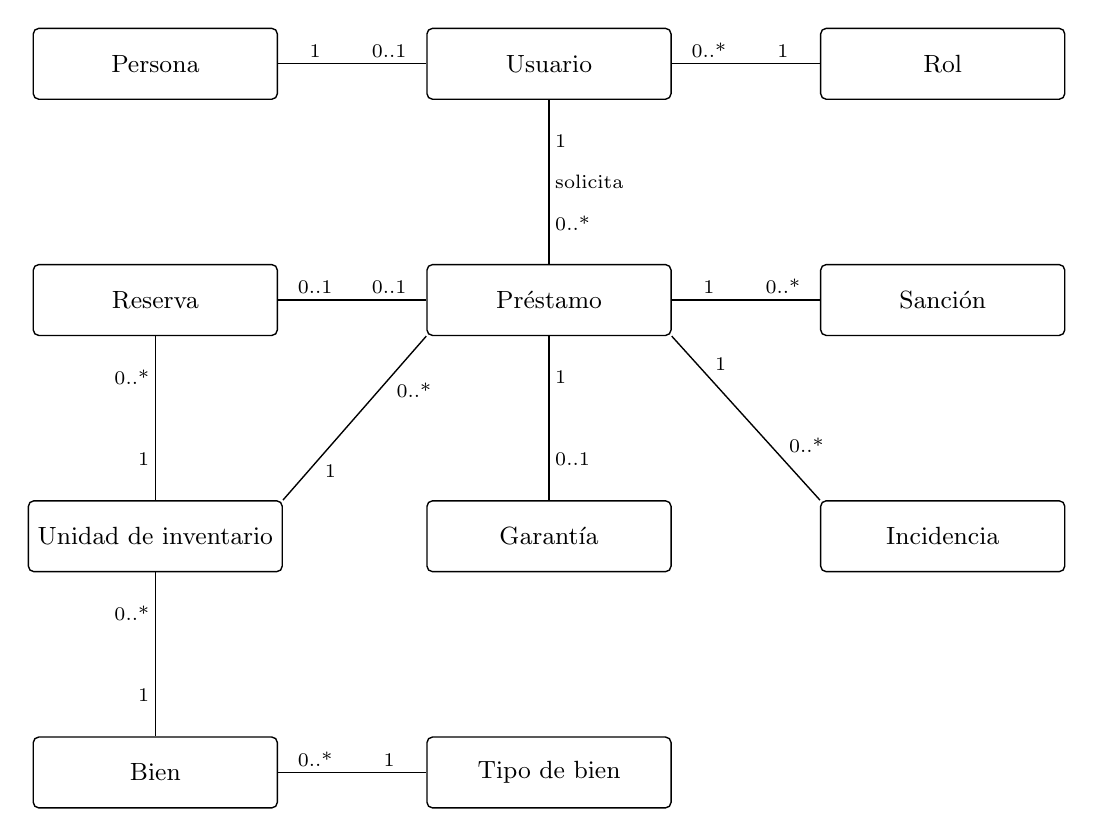
\begin{tikzpicture}[
    entidad/.style={draw,rounded corners=2pt,minimum width=3.1cm,minimum height=0.9cm,align=center,font=\small},
    cardinal/.style={font=\scriptsize,fill=white,inner sep=2pt},
    every path/.style={line width=0.5pt}
]
    \node[entidad] (persona) at (0,0) {Persona};
    \node[entidad] (usuario) at (5,0) {Usuario};
    \node[entidad] (rol) at (10,0) {Rol};
    \node[entidad] (reserva) at (0,-3) {Reserva};
    \node[entidad] (prestamo) at (5,-3) {Pr\'estamo};
    \node[entidad] (sancion) at (10,-3) {Sanci\'on};
    \node[entidad] (unidad) at (0,-6) {Unidad de inventario};
    \node[entidad] (garantia) at (5,-6) {Garant\'ia};
    \node[entidad] (incidencia) at (10,-6) {Incidencia};
    \node[entidad] (bien) at (0,-9) {Bien};
    \node[entidad] (tipo) at (5,-9) {Tipo de bien};

    \draw (persona) -- node[cardinal,near start,above]{1} node[cardinal,near end,above]{0..1} (usuario);
    \draw (usuario) -- node[cardinal,near start,above]{0..*} node[cardinal,near end,above]{1} (rol);
    \draw (usuario) -- node[cardinal,near start,right]{1} node[cardinal,midway,right]{solicita} node[cardinal,near end,right]{0..*} (prestamo);
    \draw (reserva) -- node[cardinal,near start,above]{0..1} node[cardinal,near end,above]{0..1} (prestamo);
    \draw (reserva) -- node[cardinal,near start,left]{0..*} node[cardinal,near end,left]{1} (unidad);
    \draw (unidad.north east) -- node[cardinal,near start,below right]{1} node[cardinal,near end,below right]{0..*} (prestamo.south west);
    \draw (prestamo) -- node[cardinal,near start,above]{1} node[cardinal,near end,above]{0..*} (sancion);
    \draw (prestamo) -- node[cardinal,near start,right]{1} node[cardinal,near end,right]{0..1} (garantia);
    \draw (prestamo.south east) -- node[cardinal,near start,above right]{1} node[cardinal,near end,above right]{0..*} (incidencia.north west);
    \draw (unidad) -- node[cardinal,near start,left]{0..*} node[cardinal,near end,left]{1} (bien);
    \draw (bien) -- node[cardinal,near start,above]{0..*} node[cardinal,near end,above]{1} (tipo);
\end{tikzpicture}
\caption{N\'ucleo del modelo de dominio de pr\'estamos}
\label{fig:dominio}
\end{figure}

\section{Cardinalidades y relaciones}

En la tabla, cada fila se lee desde una instancia de la entidad de origen. La multiplicidad \texttt{0..*} significa cero o muchas; \texttt{0..1}, opcional y como m\'aximo una. Las relaciones hist\'oricas no autorizan operaciones simult\'aneas incompatibles.

\begingroup
\small
\begin{longtable}{@{}>{\raggedright\arraybackslash}p{3.1cm}>{\raggedright\arraybackslash}p{3.2cm}>{\raggedright\arraybackslash}p{8cm}@{}}
\caption{Relaciones del modelo de dominio}\label{tab:relaciones}\\
\toprule
\textbf{Origen} & \textbf{Destino} & \textbf{Regla de asociaci\'on} \\
\midrule
\endfirsthead
\toprule
\textbf{Origen} & \textbf{Destino} & \textbf{Regla de asociaci\'on} \\
\midrule
\endhead
\bottomrule
\endfoot
Persona & Usuario & Una persona tiene 0..1 cuenta; cada cuenta pertenece a 1 persona. \\
Usuario & Rol & Cada usuario tiene 1 rol; un rol clasifica 0..* usuarios. \\
Usuario & Perfil & Tiene 0..1 perfil de cada tipo; el del rol solicitante actual es obligatorio. Cada perfil pertenece a 1 usuario. \\
TipoBien & Bien & Un tipo agrupa 0..* fichas; cada ficha tiene 1 tipo. \\
Bien & UnidadInventario & Una ficha describe 0..* unidades; cada unidad corresponde a 1 ficha. \\
Rol / TipoBien & PoliticaPrestamo & Cada rol o tipo puede participar en 0..* versiones; una versi\'on refiere 0..1 rol y 0..1 tipo seg\'un su alcance. \\
Usuario & Reserva & Un solicitante tiene 0..* reservas; cada reserva tiene 1 solicitante. \\
UnidadInventario & Reserva & Una unidad tiene 0..* reservas hist\'oricas; cada reserva corresponde a 1 unidad. \\
Reserva & Prestamo & Una reserva origina 0..1 pr\'estamo; un pr\'estamo procede de 0..1 reserva. No es una relaci\'on de una reserva con varios pr\'estamos. \\
Usuario & Prestamo & Como solicitante, tiene 0..* pr\'estamos; cada pr\'estamo tiene 1 solicitante. Como administrador, autoriza 0..* entregas; cada pr\'estamo tiene 1 autorizante. \\
UnidadInventario & Prestamo & Una unidad registra 0..* pr\'estamos hist\'oricos, pero como m\'aximo 1 abierto; cada pr\'estamo tiene 1 unidad. \\
Prestamo & PoliticaPrestamo & Conserva referencias a las versiones que aportan condiciones y cupo; una versi\'on puede respaldar 0..* pr\'estamos. \\
Prestamo & Renovacion & Tiene 0..* renovaciones; cada renovaci\'on pertenece a 1 pr\'estamo y tiene 1 administrador autorizante. \\
Prestamo & Garantia & Tiene 0..1 garant\'ia, obligatoria si se exige; cada garant\'ia pertenece a 1 pr\'estamo. \\
Prestamo & Sancion & Puede originar 0..* sanciones; cada sanci\'on refiere 1 pr\'estamo y a su solicitante. \\
Prestamo & Incidencia & Tiene 0..* incidencias; cada incidencia pertenece a 1 pr\'estamo. \\
Garantia & Incidencia & Puede tener 0..* incidencias; una incidencia refiere 0..1 garant\'ia del mismo pr\'estamo. \\
Usuario & EventoHistorial & Un usuario genera 0..* eventos; cada evento tiene 0..1 usuario actor, obligatorio salvo que se identifique un proceso autom\'atico. \\
\end{longtable}
\endgroup
